\section{Definitionen}



Information Gap:
\cite{dervin2003sense}
sense-making incorporates a repertoire of potenteial procedures for accomplishing the goals discussed preciously. All these are drawn from a xenral metaphor, shown in Figure 12.2 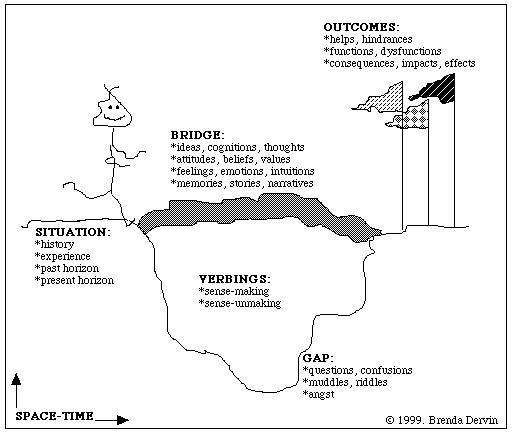
\includegraphics[width=00.5]{SMM_MEtaphor.jpg}. Here, one sees a human moving across time and space, facing a gap, building a bridge across the gap, and then constructing and evaluating the uses of the bridge. This metaphor rests on a descontinuity assumption - that gappiness is pervasive both in and between moments in time and space and in and between people. Gappiness is assumed to occur because of differences across time (e.g. self today vs self yesterday and scientific fact today vs. scientific fact tomorrow) and across space (e.g. the experiece of a particular condition on different cultures, contexts, communites, material circumstances and the sense of an experience physically and the articulation of it verbally)
continue on Dervin p.238

Informationslücke

Geflüchteter
refugee:
Firstly, the key word in the UN convention is “persecution”
but it has no single definition. Persecutions can be for
various reasons as defined by the host country and the
scope of persecutions for each host country keeps
expanding and evolving with time. Secondly, there are
numerous routes of arrival into the host country integration
systems. This is alongside the earlier highlighted categories
of persons in the integration system. Refugee integration is
indeed a complicated phenomenon, a situational
information behaviour approach is the only chance that all
the variables in the complexity will be factored into the
understanding.

Asylsuchender

Integration
Oduntan
The UN convention is operated in an asylum system in
which refugees arrive under different elements. The
systems incorporate varied levels of access to provisions
including support, benefits, work entitlements and rights to
remain. Thus refugee integration starts on arrival in the host
country through the transition process.



refinition refugee Hannah Arendt VS UN?

Hannah Arendt: 'in the first place, we don't like to be called "refugees". We ourselves call each other "newcomers" or "immigrants." [..] A refugee used to be a person driven to seek refuge because of some act committed or some political opinion held. Well, it is true we have had to seek refuge; but we committed no acts and most of us never dreamt of having any radical opinion. With us the meaning of the term “refugee” has changed. Now “refugees” are those of us who have been so unfortunate as to arrive in a new country without means and have to be helped by Refugee Committees.
[..]Yes, we were “immigrants” or “newcomers” who had left our country because, one fine day, it no longer suited us to stay, or for purely economic reasons. We wanted to rebuild our lives, that was all. In order to rebuild one’s life one has to be strong and an optimist. So we are very optimistic. [..]
We lost our home, which means the familiarity of daily life. We lost our occupation, which means the confidence that we are of some use in this world. We lost our language, which means the naturalness of reactions, the simplicity of gestures, the unaffected expression of feelings. We left our relatives in the Polish ghettos and our best friends have been killed in concentration camps, and that means the rupture of our private lives.
Nevertheless, as soon as we were saved—and most of us had to be saved several times—we started our new lives and tried to follow as closely as possible all the good advice our saviors passed on to us. We were told to forget; and we forgot quicker than anybody ever could imagine.
[..] Apparently nobody wants to know that contemporary history has created a new kind of human beings—the kind that are put in concentration camps by their foes and in internment camps by their friends.

[..]have had such curious notions as to believe that we are not only “prospective citizens” but present “enemy aliens.” In daylight, of course, we become only “technically” enemy aliens—all refugees know this. But when technical reasons prevented you from leaving your home during the dark house, it certainly was not easy to avoid some dark speculations about the relation between technicality and reality.
%Bürger zweiter Klasse?
[..]Once we could buy our food and ride in the subway without being told we were undesirable.[..]We wonder how it can be done; we already are so damnably careful in every moment of our daily lives to avoid anybody guessing who we are, what kind of passport we have, where our birth certificates were filled out—and that Hitler didn’t like us. 
%Rassismus auf der Straße
[..] since passports or birth certificates, and sometimes even income tax receipts, are no longer formal papers but matters of social distinction.
%Nicht in die Disco gelassen

The comity of European peoples went to pieces when, and because, it allowed its weakest member to be excluded and persecuted.